
\section{Placement}
\label{sec:placement}
So far we have only dealt with technology problems where we consider the problem space and adress the constraints of the hardware architecture. 
For every constraint, we devise a solution or a simplification to reduce the complexity of the problem space. 

Now that we have dealt with the bulk of these constraints and squared them away into self-contained \texttt{SiteInst}s, we can now apply some general optimization algorithms to finally address our optimization objective, which is to place these \texttt{SiteInst}s onto the device while minimizing wirelength. 

In this paper we implement and present a Simulating Annealing (SA) placer that operates at the \texttt{SiteInst} level. 



\subsection{Simulated Annealing}
\label{subsec:simulated_annealing}

\begin{lstlisting}[language=java, caption={Simulated Annealing pseudocode}, label={lst:sa_pseudocode}]
public void placeDesign(PackedDesign packedDesign) {
    // unplace the pseudorandom packed placement
    unplaceAllSiteInsts(packedDesign);
    // place randomly
    randomInitialPlacement(packedDesign);
    int moves = 0;
    while (moves < 300) {
        move(packedDesign)
        updateTemperature();
        moves++;
    }
}

private void move(PackedDesign packedDesign) {
    moveSiteChains(packedDesign.DSPSiteInstCascades);
    moveSiteChains(packedDesign.CARRYSiteInstChains);
    moveSingleSite(packedDesign.RAMSiteInsts);
    moveSingleSite(packedDesign.CLBSiteInsts);
}

protected void moveSingleSite(List<SiteInst> sites) {
    for (SiteInst si : sites) {
        // We refer to the current Site si as the "home site"
        // We refer to the proposed Site as the "away site"

        // Find the list of Sites connected to the home site
        List<Site> homeConns = findConnectedSites(si);

        Site homeSite = si.getSite();
        // Select an away site (random selection, midpoint, centroid, etc.)
        Site awaySite = proposeSite();

    }
}

protected void moveSingleSite(List<SiteInst> sites) {
    for (SiteInst si : sites) {
        SiteTypeEnum ste = si.getSiteTypeEnum();
        List<Site> homeConns = findConnectedSites(si, null);
        Site homeSite = si.getSite();
        Site awaySite = proposeSite(si, homeConns, true);
        SiteInst awaySi = occupiedSites.get(ste).get(awaySite);
        double oldCost = 0;
        double newCost = 0;
        if (awaySi != null) {
            List<Site> awayConns = findConnectedSites(awaySi, null);
            oldCost += evaluateSite(homeConns, homeSite);
            oldCost += evaluateSite(awayConns, awaySite);
            newCost += evaluateSite(homeConns, awaySite);
            newCost += evaluateSite(awayConns, homeSite);
        } else {
            oldCost += evaluateSite(homeConns, homeSite);
            newCost += evaluateSite(homeConns, awaySite);
        }
        if (evaluateMoveAcceptance(oldCost, newCost)) {
            if (awaySi != null) {
                unplaceSiteInst(si);
                unplaceSiteInst(awaySi);
                placeSiteInst(si, awaySite);
                placeSiteInst(awaySi, homeSite);
            } else {
                unplaceSiteInst(si);
                placeSiteInst(si, awaySite);
            }
        }
    }
} // end randomMoveSingleSite()
\end{lstlisting}


{
    \centering
    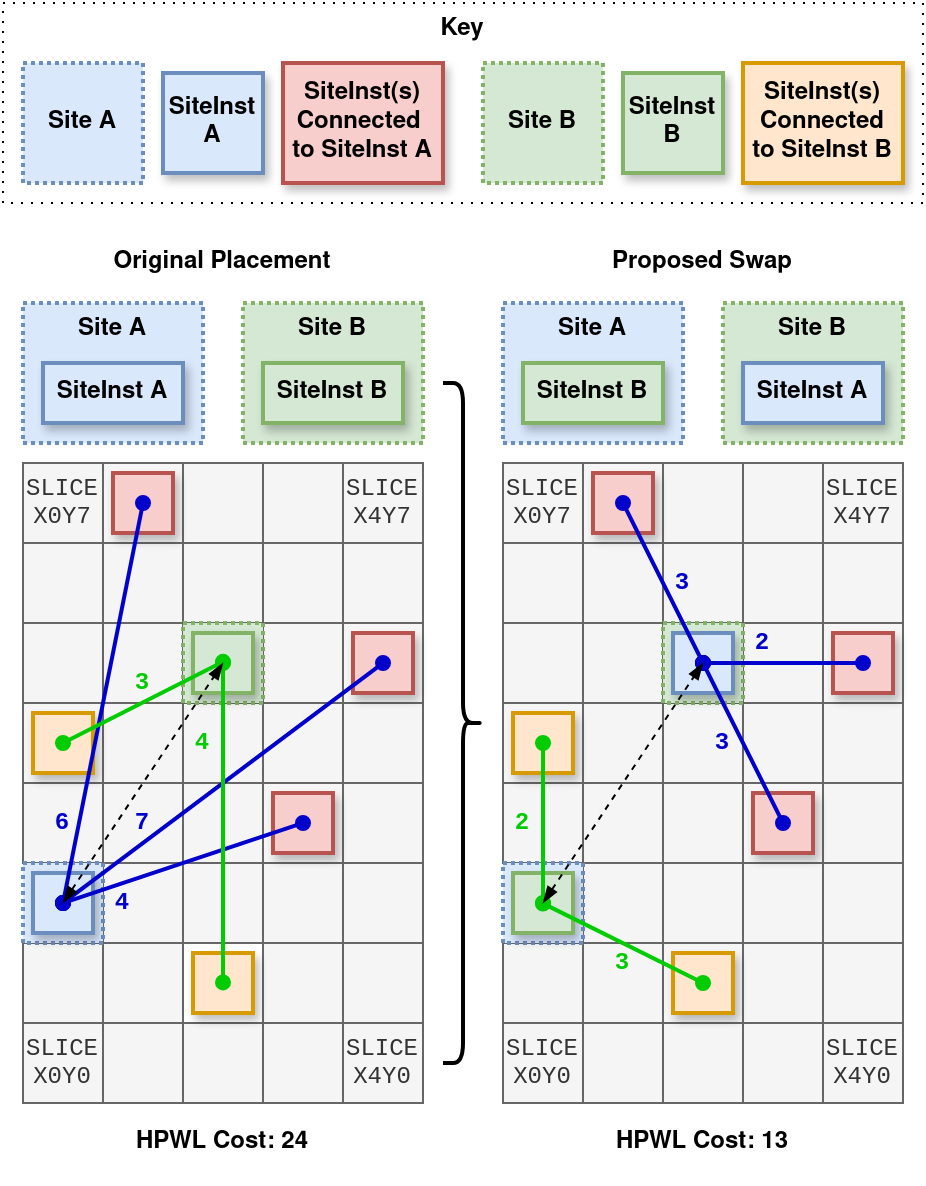
\includegraphics[width=\columnwidth]{figures/placement/swapSingleSite.png}
    \captionof{figure}{Single Site Swap Proposal}
    \label{fig:swapSingleSite}
}

\begin{lstlisting}[language=java, caption={Chain Swapping}, label={lst:chain_swap_pseudocode}]
protected void moveSiteChains(List<List<SiteInst>> chains) {
for (List<SiteInst> current_chain : chains) {
    int ch_size = current_chain.size();
    /*

    1) Draw a vertical window of equal size to the current chain. We will refer to this window as the "home window". 
    2) Select a new candidate anchor for this chain.
    2) Project the home window onto the candidate anchor with anchors coinciding. We will refer to this projected window as the "away window".
    3) Check if there are any resident SiteInsts or SiteInst chains present in the away window. Check if the away window breaks any resident SiteInst chains. 
    4)  IF (the away window breaks any chains): 
            extend the window in either direction to 
            fully accommodate all resident chains. 
        ELSE: GOTO evaluateMove(). 
    5) Project the extended away window back onto the original region with the tail of the window coinciding with the tail of the current chain. This projected window becomes the new home window. 
    7) WHILE (the home window breaks any resident chains):
        shift the window upwards by one Site. 
        IF (number of shifts > home window size - ch_size):
            reject the candidate swap.
            CONTINUE onto next chain
    8) evaluateMove(): HPWL Cost evaluation 
    9) evaluateMoveAcceptance(): hill-climb acceptance with global temperature

    */
}
}
\end{lstlisting}

\newpage
\end{multicols}
{
    \centering
    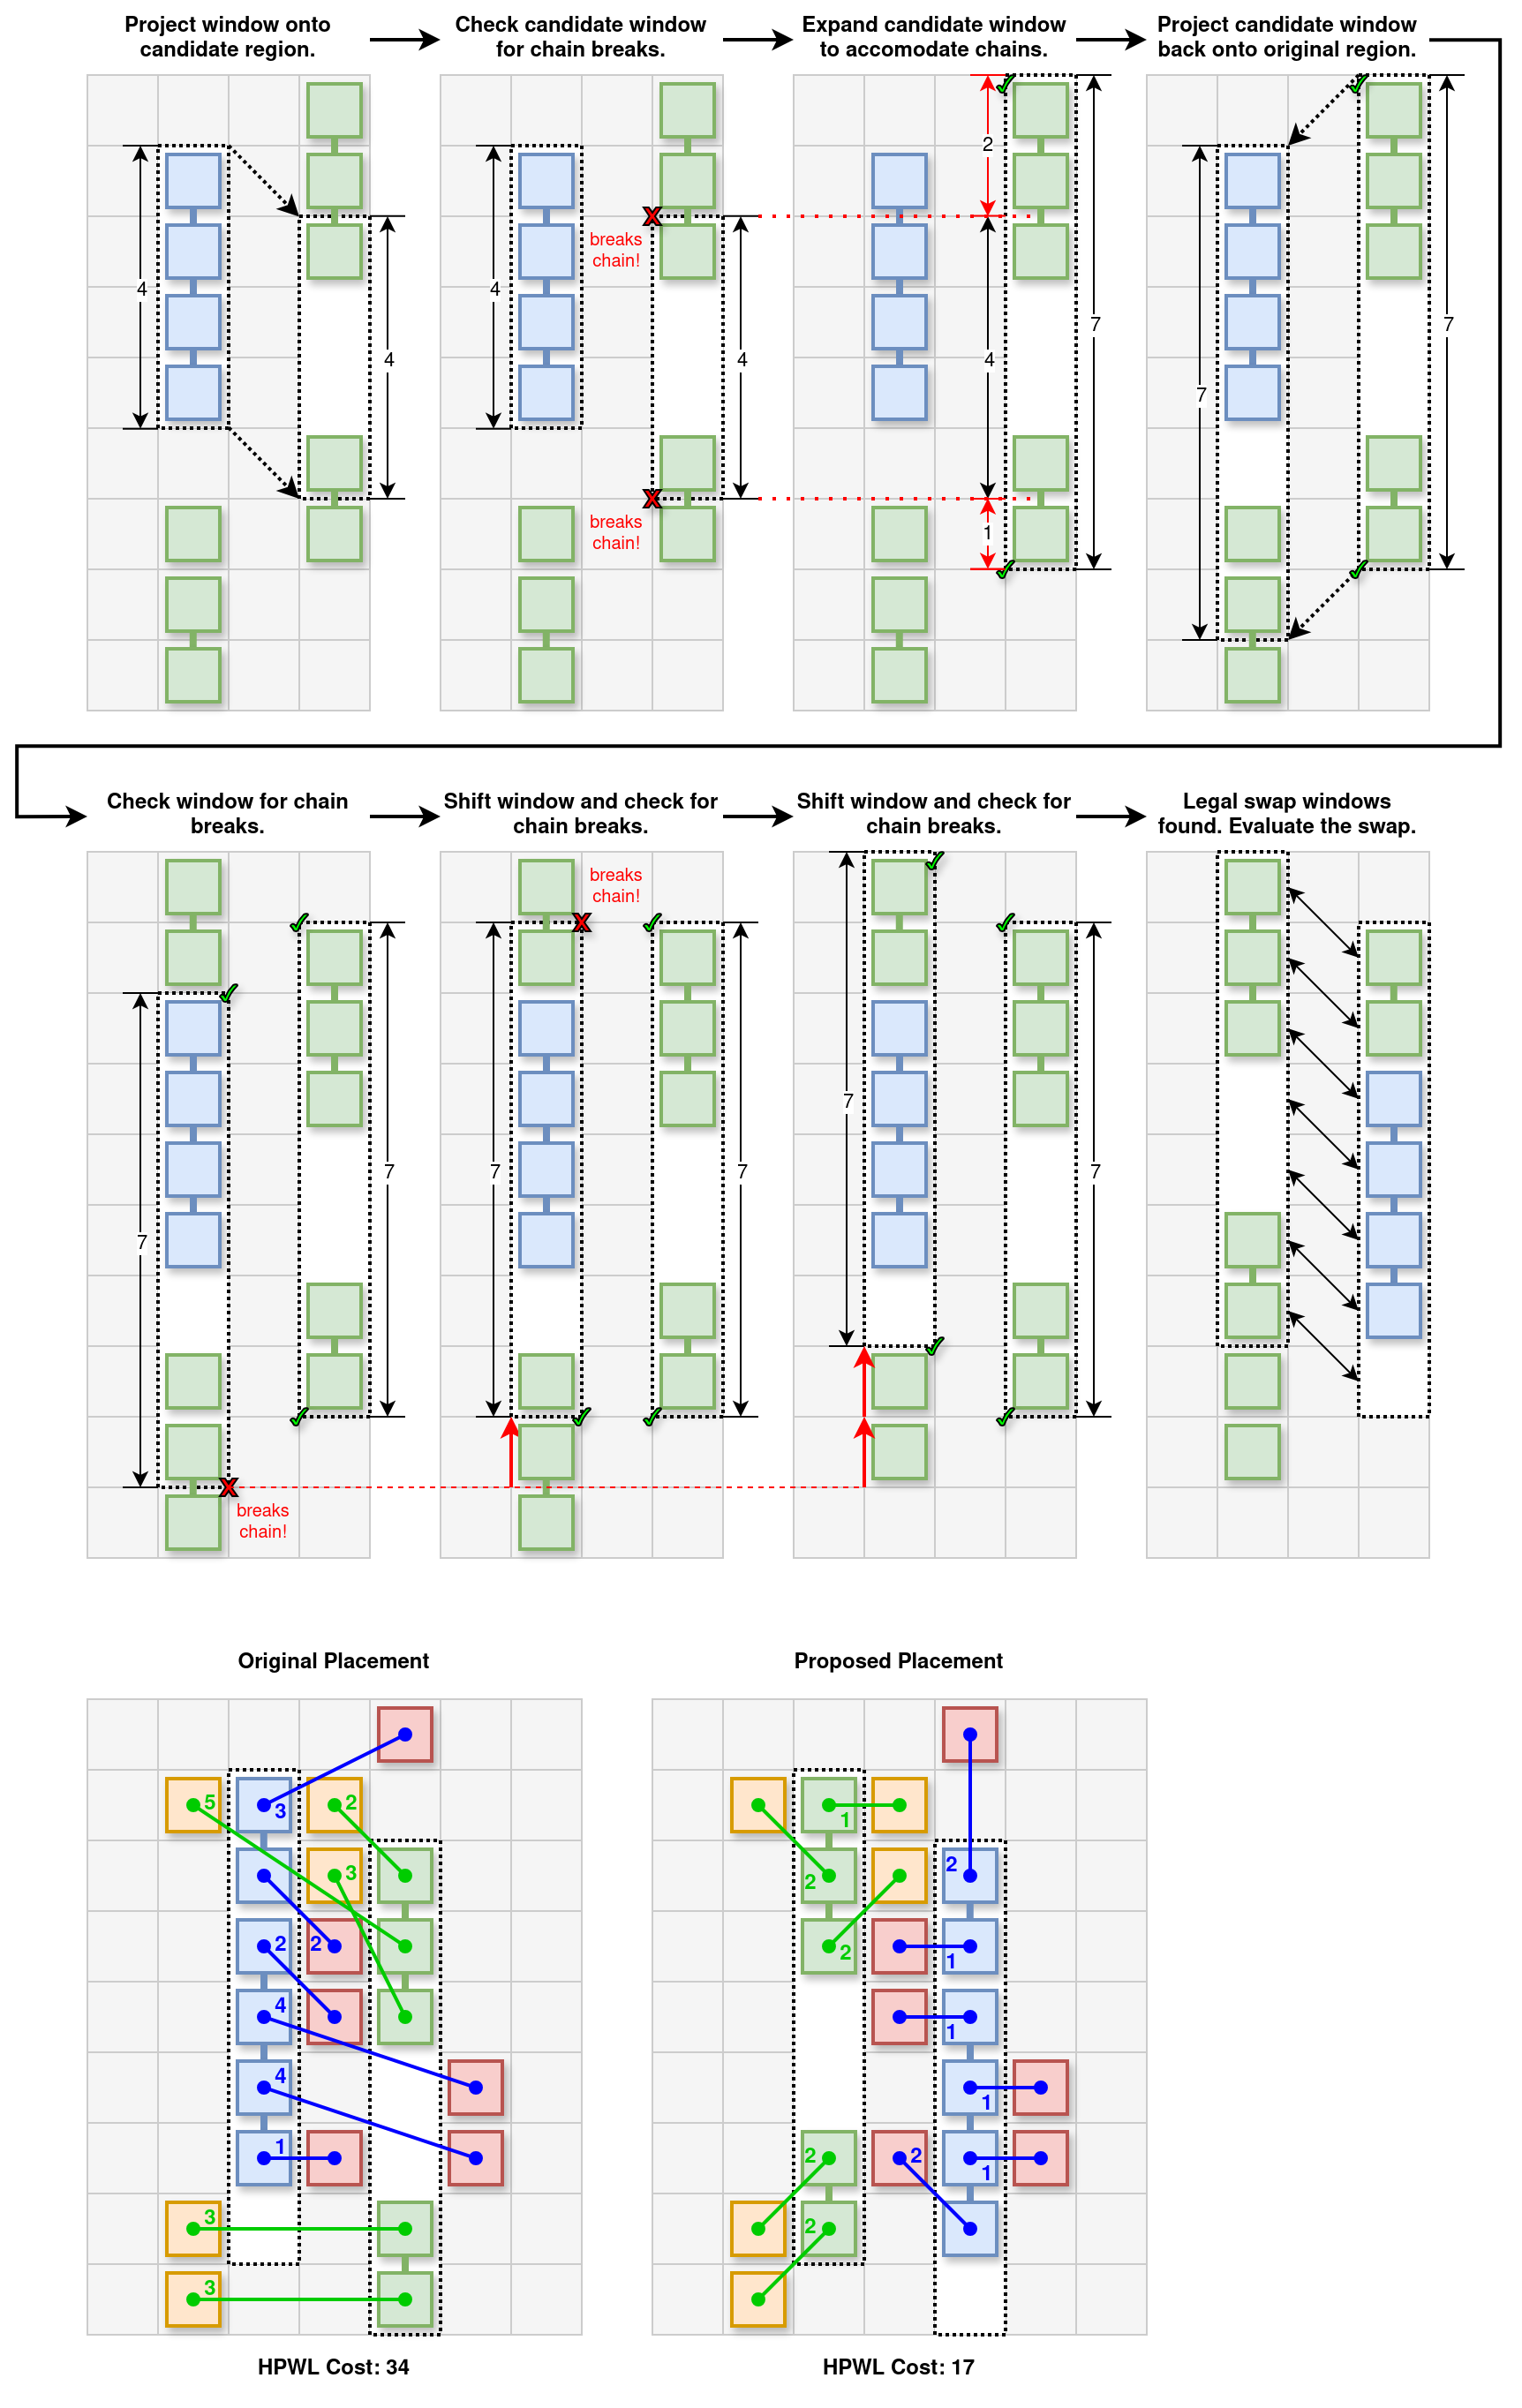
\includegraphics[width=0.9\columnwidth]{figures/placement/swapSiteChain.png}
    \captionof{figure}{Site Chain Swap Proposal}
    \label{fig:swapChainSite}
}
\begin{multicols}{2}

Select a new anchor Site.
Project a window onto the proposed Site
If the window anchor breaks a chain, extend the window in its direction until the anchor coincides with the chain anchor..
If the window tail breaks a chain, extend the window in its direction until the tail coincides with the chain tail.



